\documentclass[11pt]{beamer}

\usetheme{Oxygen}
\usepackage{xcolor}
\usepackage{thumbpdf}
\usepackage{wasysym}
\usepackage[utf8]{inputenc}
\usepackage[brazil]{babel}
\usepackage{graphicx}
\usepackage{pgf,pgfarrows,pgfnodes,pgfautomata,pgfheaps,pgfshade}
\usepackage{verbatim}

%\useoutertheme{shadow}
\setbeamertemplate{sections/subsections in toc}[sections numbered]
\setbeamersize{text margin left=10mm}
\setbeamersize{text margin right=8mm}

\definecolor{laranja}{HTML}{cc0000}
\definecolor{azul}{HTML}{003366}

%\setbeamercolor{alerted text}{fg=azul}
%\setbeamercolor{structure}{fg=azul}
%\setbeamercolor{palette primary}{fg=laranja}
%\setbeamercolor{palette secondary}{fg=laranja!75!black}
%\setbeamercolor{palette tertiary}{fg=laranja!50!black}
%\setbeamercolor{palette quaternary}{fg=black}

\def\gap{\vspace{0.1in}}
\def\Gap{\vspace{0.25in}}

\pdfinfo {
	/Title   (Wiki UFC)
	/Creator (TeX)
	/Author  (Álinson Santos,
	          André Castro,
			  Adriano Freitas,
	          Luis Henrique,
			  Rafael Barbosa)
}


\title{\textbf{Wiki UFC}}
\subtitle{Apresentação da Aplicação}
\date{28 de junho de 2007}
\author[Álinson, André, Adriano, Bustamante, Rafael]{\small{
	Álinson Santos  \\
	André Castro    \\
	Adriano Freitas \\
	Luis Henrique   \\
	Rafael Barbosa
}}

\begin{document}

% Capa
% ==============================================================================
\section*{}
\frame{
	\titlepage
	\thispagestyle{empty}
}
\begin{frame}
	\frametitle{Índice}
	%\framesubtitle{Visão geral}
	\tableofcontents[subsectionstyle=hide]
\end{frame}

\AtBeginSection[] {
	\frame<handout:0> {
		\frametitle{Índice}
		%\framesubtitle{\insertsection}
		\tableofcontents[currentsection,subsectionstyle=show/show/hide]
	}
}

%\AtBeginSubsection[] {
%	\frame<handout:0> {
%		\tableofcontents[sectionstyle=show/hide,subsectionstyle=show/shaded/hide]
%	}
%}

\newcommand<>{\highlighton}[1]{%
	\alt#2{\structure{#1}}{{#1}}
}


% Introdução
% ==============================================================================
\section{Introdução}

	% Problema atual e solucao proposta
	% -------------------------------------------------------------------------
	\subsection{Problema atual}
	\begin{frame}
		\frametitle{Problema atual}

		Hoje em dia, os alunos do nosso curso não possuem uma maneira eficiente
		de trocar informações sobre as disciplinas que estão cursando.

		\gap
		\begin{itemize}
			\item Cada disciplina possui sua própria lista de emails
			\item Não existe um calendário oficial no qual os estudantes possam
			confiar
			\item É dificil compartilhar material como notas de aulas e listas
			de exercícios
			\item É díficil obter o material utilizado nos semestres anteriores
		\end{itemize}
	\end{frame}

	% Objetivos
	% -------------------------------------------------------------------------
	\subsection{Solução proposta}
	\begin{frame}
		\frametitle{Solução proposta}
		Uma aplicação \textsc{WEB} colaborativa onde os alunos poderão
		compartilhar informações sobre as disciplinas que estão cursando.

		\Gap
		Objetivos:
		\begin{itemize}
			\item Permitir a colaboração descentralizada de alunos para o curso
			\item Facilitar a divulgação do conhecimento
			\item Tornar a vida do estudante mais organizada
		\end{itemize}

	\end{frame}

	% Soluções alternativas
	% -------------------------------------------------------------------------
	\subsection{Soluções alternativas}
	\begin{frame}
		\frametitle{Soluções alternativas}

		\begin{block}{WebAdmin}
			Sistema criado por Windson Viana para facilitar a manutenção de
			páginas pelos professores do curso de Computação. Em funcionamento
			no site \texttt{http://disciplinas.lia.ufc.br}
		\end{block}

		\gap
		\begin{block}{Moodle}
			Moodle é um Software Livre de E-Learning, desenvolvido para
			facilitar a criação de cursos online não presencias. Possui recursos
			avançados, como fóruns, blogs, wikis, chats, e quizzes.
		\end{block}
	\end{frame}

% Metodologia
% ==============================================================================
\section{Metodologia}

	\begin{frame}
		\frametitle{Scrum}
		Scrum é um método ágil, criado em 1993, para permitir
		que o desenvolvimento rápido de aplicações. Atualmente é utilizado
		em empresas como Google, Yahoo, Eletronic Arts, Philips e Nokia.

		\Gap
		Como funciona?

		\begin{itemize}
			\item Manutenção de um \alert{backlog}, com as tarefas pendentes
			\item Desenvolvimento segmentado em ciclos, chamados de \alert{sprints}
			\item Reuniões periódicas, ao final de cada sprint
		\end{itemize}
	\end{frame}

	\begin{frame}
		\frametitle{Scrum}
		\framesubtitle{Backlog}
		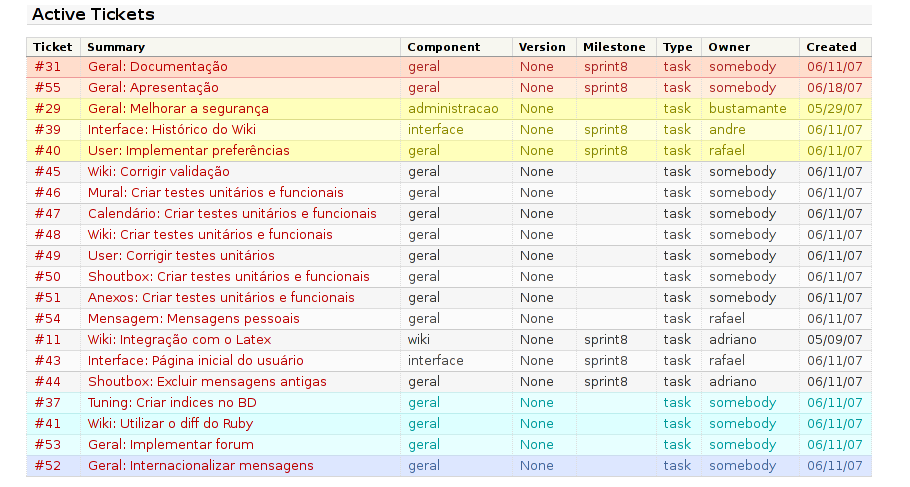
\includegraphics[width=110mm]{backlog.png}
	\end{frame}
	\begin{frame}
		\frametitle{Scrum}
		\framesubtitle{Sprints e Reuniões}

		No nosso projeto,
		\begin{itemize}
			\item Cada sprint durava uma semana
			\item As reuniões eram realizadas segundas feiras, às 16h
		\end{itemize}

		\gap
		Em cada reunião:
		\begin{itemize}
			\item Discutíamos o que havia sido implementado no sprint anterior
			\item Discutíamos o que não havia sido implementado, por algum
			motivo..
			\item Colocávamos novos itens no backlog
			\item Definiamos que tarefas cada um realizaria durante o próximo
			sprint
		\end{itemize}
	\end{frame}


% Tecnologias
% ==============================================================================
\section{Tecnologias}

	% Ruby
	% --------------------------------------------------------------------------

	\subsection{Linguagem Ruby}
	\begin{frame}
		\frametitle{Linguagem Ruby}
		Ruby é uma linguagem de programação orientada a objetos, criada por
		Yukihiro Matsumoto em 1995. Implementação oficial licenciada sob a GPL.

		\gap
		\begin{itemize}
			\item Sintaxe simples e legível
			\item Completamente orientada a objetos
			\item Herança múltipla avançada, através de Mixins
			\item Introspecção, reflexão e meta-programação
			\item Garbage collector
		\end{itemize}
	\end{frame}


	% Ruby on Rails
	% --------------------------------------------------------------------------
	\subsection{Ruby on Rails}
	\begin{frame}
		\frametitle{Ruby on Rails}
		Ruby on Rails é um framework para o desenvolvimento aplicações web, que
		segue os principios \emph{Don't Repeat Yourself (DRY)} e
		\emph{Convention over Configuration}.

		\gap
		\begin{columns}[c] 
		\column{1.0in}
			\begin{center}
				
\includegraphics[width=0.60 in]{rails.png}
			\end{center}
		\column{5.5in}
			\begin{itemize}
				\item Arquitetura Model-View-Controller
				\item Mapeamento objeto-relacional
				\item Scaffolds, Generators e Migrations
				\item Suporte nativo a testes automatizados
				\item Integração com Ajax e Webservices
				\item Servidor web incluso!
			\end{itemize}
		\end{columns}
	\end{frame}

	\begin{frame}
		\frametitle{Ruby on Rails}
		\framesubtitle{A arquitetura MVC}
		\begin{description}
		\item Arquitetura para desenvolvimento que trabalha com três partes:
		\item[Model] Dados armazenados da aplicação
		\item[View] Seção visível ao usuário, e com a qual ele interage
		\item[Controller] Interface entre Model e View, que estabelece as regras de negócio.
		\end{description}
	\end{frame}
%
%	\begin{frame}
%		\frametitle{Rails é ágil!}
%		\begin{itemize}
%			\item Para um desenvolvimento ágil...
%			\item ... é necessária uma "linguagem ágil"\vspace{2mm}
%			\item Rails é ágil!\vspace{4mm}
%			\item Com Rails, é possível fazer um blog em 15 minutos: \\ http://www.rubyonrails.org/screencasts
%		\end{itemize}
%		\framesubtitle{Um blog em 15 minutos}
%	\end{frame}

	% Subversion e Trac	
	% --------------------------------------------------------------------------
	\subsection{Subversion e Trac}
	\begin{frame}
		\frametitle{Subversion e Trac}
		Subversion é um software open source para controle de versões.
		\begin{itemize}
			\item O código fonte é armazenado em um servidor web
			\item Cada programador pode ler e modificar os arquivos remotamente
			\item As versões antigas dos arquivos estão sempre disponíveis para
			consulta.
		\end{itemize}

		\gap
		Trac é uma aplicação web para gerenciamento de projetos e bugtracking,
		com integração a Subversion.
	\end{frame}

% Aplicação
% ==============================================================================
\section{Aplicação}

	% Funcionalidades
	% --------------------------------------------------------------------------
	\subsection{Funcionalidades}
	\begin{frame}
		\frametitle{Funcionalidades}

		Entre as funcionalidades implementadas estão:

		\gap
		\begin{itemize}
			\item Um \textsc{Wiki} para conter as notas de aula
			\item Um calendário, para receber datas de provas e entregas de
			trabalho
			\item Um repositório de arquivos, onde serão armazenadas listas de
			exercícios, e provas antigas
			\item Um mural, para postagem de notícias sobre a disciplina
		\end{itemize}
	\end{frame}

	\begin{frame}
		\frametitle{Funcionalidades}
		\framesubtitle{Adicionais}

		E, além das funcionalidades básicas:

		\gap
		\begin{itemize}
			\item Wiki com suporte a sintaxe Markdown e controle de versões,
			\item Calendário com exportação nos formatos iCalendar e RSS,
			\item Shoutbox, que permite a comunicação rápida entre os usuários,
			\item Página pessoal, que integra as informações sobre as disciplinas cursadas pelo
			aluno,
			\item Site personalizável.
		\end{itemize}
	\end{frame}

	% Demonstração
	% --------------------------------------------------------------------------
	\subsection{Demonstração}
	\begin{frame}
		\frametitle{Wiki UFC}
		\begin{center}\alert{Demonstração...}\end{center}
	\end{frame}

% Conclusão
% ==============================================================================
\section{Conclusão}

	% Dificuldades Encontradas
	% --------------------------------------------------------------------------
	\subsection{Dificuldades Encontradas}
	\begin{frame}
		\frametitle{Dificuldades encontradas}
		As maiores dificuldades para realizar o projeto foram:

		\gap
		\begin{itemize}
			\item Estudar a linguagem Ruby
			\item Aprender a utilizar os recursos do framework Ruby on Rails
			\item Conseguir tempo para programar, já que nós estamos cursando,
			pelo menos, quatro outras disciplinas
			\item Sincronizar o nosso método ágil com relatórios tradicionais da
			disciplina
		\end{itemize}	
	\end{frame}


	% Pontos Positivos
	% --------------------------------------------------------------------------
	\subsection{Pontos Positivos}
	\begin{frame}
		\frametitle{Pontos positivos}
		Sobre o projeto em geral:
		\begin{itemize}
			\item A equipe aprendeu a utilizar muitas tecnologias novas
			\item Aplicamos alguns conceitos da disciplina na prática
		\end{itemize}	
		
		\gap
		Sobre o método Scrum:
		\begin{itemize}
			\item Reuniões semanais: não ficou tudo pro fim!
			\item Backlog: Sabíamos exatamente o que ainda faltava ser feito
		\end{itemize}
	\end{frame}

	% Perspectivas
	% --------------------------------------------------------------------------
	\subsection{Perspectivas}
	\begin{frame}
		\frametitle{Perspectivas}
		Para o futuro, planejamos:

		\gap
		\begin{itemize}
			\item Implementar alguns itens que, por falta de tempo, não puderam
			ser inclusos no projeto original.
			\item Colocar em funcionamento, para os alunos puderem usar de
			verdade.
			\item Abrir como um projeto Open Source.
		\end{itemize}
	\end{frame}

% Perguntas?
% ==============================================================================
\begin{frame}
	\frametitle{Fim!}
	\begin{center}\huge{\alert{Perguntas?}}\end{center}
\end{frame}

\end{document}
